\documentclass{beamer}
\usepackage{amssymb}
\usepackage{graphicx}
\usetheme{default}
\author{Bart Offereins\\Marco Gunnink}
\title{Raytracing exercize 1,2}

\begin{document}

\titlepage

\begin{frame}{Ray sphere intersection}

\begin{itemize}
  \item abc-formula, but with vectors
  \item dot product $\rightarrow$ discriminant is a single value
  \item discriminant $<$ 0, no hit
  \item abc formula results in distances intersect-ray origin, pick shortest
\end{itemize}

\end{frame}

\begin{frame}{Normal calculation}

\begin{itemize}
  \item Normal vector is at right angle to surface
  \item Radius is at right angle to surface
  \item Radius direction $==$ Normal direction 
  \item Intersect point $-$ sphere position
\end{itemize}

\end{frame}

\begin{frame}{Phong illumination}

\begin{itemize}
  \item Three components
  \item Ambient: factor to material and light color
  \item Diffuse: factor to material and light color, involves Normal vector, must be $> 0$
  \item Specular: Nothing to do with material color !!
\end{itemize}

   \begin{figure}[ht]
       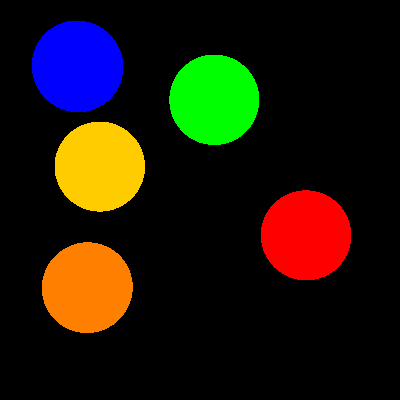
\includegraphics[width=5cm]{scene01.png} %phong wrong
       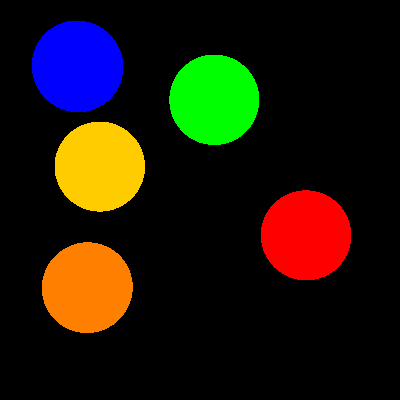
\includegraphics[width=5cm]{scene01.png} %phong right
    \end{figure}

\end{frame}




\end{document}